\documentclass[11pt,letterpaper]{article}
\usepackage[margin=0.75in]{geometry}
\usepackage{parskip}
\usepackage[section]{placeins}
\usepackage{float}
\linespread{1.0}
\usepackage[T1]{fontenc}
\usepackage{lmodern}
\usepackage{microtype}
\usepackage{booktabs,tabularx,array}
\usepackage{amsmath}
\usepackage{xcolor}
\usepackage{tikz}
\usetikzlibrary{arrows.meta,positioning,shapes.geometric}
\definecolor{evidenceblue}{HTML}{245B83}
\definecolor{decisiongreen}{HTML}{28604A}
\definecolor{reviewamber}{HTML}{785217}
\tikzset{
  evidence/.style={draw=evidenceblue,fill=evidenceblue!5},
  decision/.style={draw=decisiongreen,fill=decisiongreen!5},
  review/.style={draw=reviewamber,fill=reviewamber!7},
  paperbox/.style={rounded corners=2pt,align=left,font=\small,
    inner sep=7pt,line width=0.65pt},
  flowarrow/.style={-{Latex[length=2mm]},line width=0.75pt}
}
\usepackage[hidelinks]{hyperref}
\usepackage{url}
\urlstyle{same}
\newcommand{\run}[1]{\texttt{\detokenize{#1}}}
\newcommand{\pending}{\textit{Pending}}
\setlength{\emergencystretch}{1.5em}
\title{NP Labs at TRECVID 2026: Video Answer Generation\\and Multiple-Choice Ranking}
\author{Nidhin Pattaniyil\\Individual participant (team: NP Labs)}
\date{}

\newcolumntype{Y}{>{\raggedright\arraybackslash}X}
\begin{document}
\begin{center}
{\Large\bfseries NP Labs at TRECVID 2026:\\Video Answer Generation and Multiple-Choice Ranking\par}
\vspace{8pt}
Nidhin Pattaniyil\\Individual participant (team: NP Labs)
\end{center}
\section*{Structured Abstract}
\textbf{Data.} We used pretrained models without fine-tuning. Labeled 2025 examples guided development; correct test answers were not used for generation or ranking. All eight submissions cover 2,443 questions from 1,956 videos. Official scoring covers 2,428 questions after 15 exclusions.

\textbf{Answer Generation (AG).} AG1 answers from 12 video frames. AG2 combines Qwen video answers with and without a Whisper speech transcript. AG3 puts Gemini's audio-video answer first, then Qwen alternatives. AG4 groups and rewords saved answers while keeping AG3's first answer fixed.

\textbf{Multiple Choice (MC).} MC1 matches our saved AG3 answer to the supplied options. MC2 uses saved video rankings where a text check flags a weak match. MC3 uses Gemini 3.7 video rankings wherever valid; MC4 follows the same approach with Gemini 3.8.

\textbf{Results.} AG3/AG4 lead METEOR@1 (.318 versus .171--.189); AG1 narrowly leads STS and AG2 BERTScore. MC accuracy rises from 78.748\% for saved-answer matching to 84.514\% for full Gemini 3.7 video ranking. Gemini 3.8 scores 84.308\%.

\textbf{Component evidence.} Adding Whisper to the same Qwen3.5 frame inputs raises token F1 from .431 to .507 on 30 development questions. This is not an ablation of the submitted AG2 configuration. Using video rankings more broadly adds 27 correct choices over MC2's targeted use of the same predictions.

\textbf{Lessons.} Video ranking corrects errors but creates others. AG4's changed lists score lower on NDCG despite preserving rank one. The worked example shows why different wording, different meanings, and different option choices must be distinguished.

\section*{Two outputs from the same question}
\begin{figure}[H]\centering
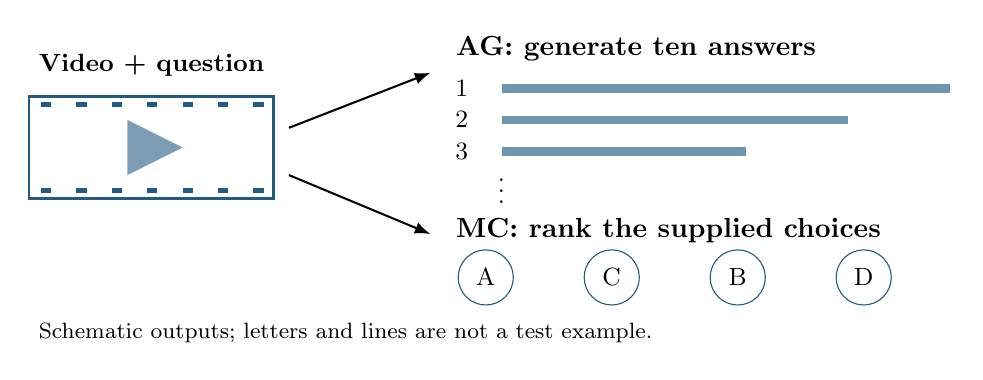
\begin{tikzpicture}[font=\small]
\node[anchor=west] at (0,2.4) {\textbf{Video + question}};
\draw[evidenceblue,line width=1pt] (0,.7) rectangle (3.1,2);
\foreach \x in {.15,.6,1.05,1.5,1.95,2.4,2.85} {
 \fill[evidenceblue] (\x,1.86) rectangle +(0.13,.07);
 \fill[evidenceblue] (\x,.77) rectangle +(0.13,.07);}
\fill[evidenceblue!60] (1.25,1) -- (1.25,1.7) -- (1.95,1.35)--cycle;
\draw[flowarrow] (3.3,1.6)--(5.1,2.3);
\draw[flowarrow] (3.3,1)--(5.1,.25);
\node[anchor=west,font=\bfseries] at (5.3,2.6) {AG: generate ten answers};
\foreach \y/\r/\w in {2.1/1/5.7,1.7/2/4.4,1.3/3/3.1} {
 \node[anchor=east] at (5.7,\y) {\r};
 \draw[evidenceblue!65,line width=3pt] (6,\y)--+(\w,0);}
\node at (6,.9) {$\vdots$};
\node[anchor=west,font=\bfseries] at (5.3,.3) {MC: rank the supplied choices};
\foreach \x/\t in {5.8/A,7.4/C,9/B,10.6/D} {
 \node[circle,draw=evidenceblue,minimum size=7mm] at (\x,-.3) {\t};}
\node[anchor=west,font=\footnotesize] at (0,-1) {Schematic outputs; letters and lines are not a test example.};
\end{tikzpicture}
\caption{AG creates answer text; MC orders the organizer's revised options~\cite{guidelines2026,smeaton2006}. Our MC1 uses an answer generated before seeing those options.}
\end{figure}

\clearpage
\section{How the submissions are built}
\subsection{AG: generate independently, then assemble}
Each source receives the question. The four sources generate independently; the submission rules below assemble their saved text.
\begin{figure}[H]\centering
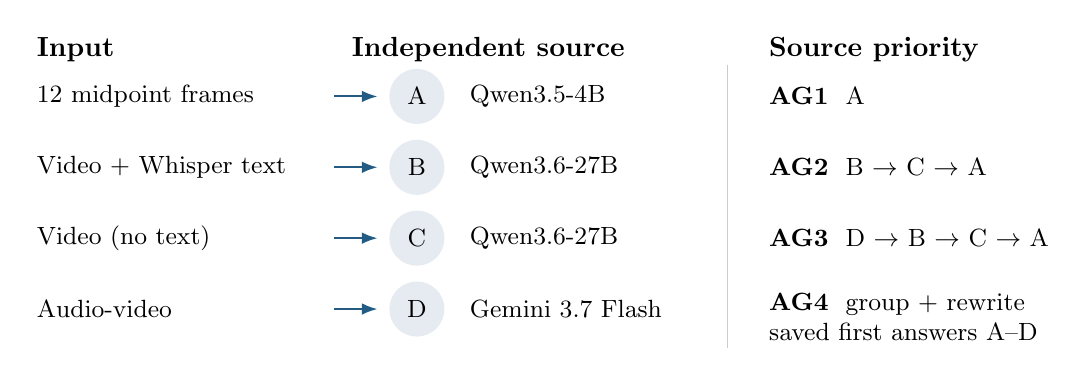
\begin{tikzpicture}[font=\small]
\node[anchor=west,font=\bfseries] at (0,.6) {Input};
\node[anchor=west,font=\bfseries] at (4,.6) {Independent source};
\foreach \y/\letter/\input/\model in {0/A/12 midpoint frames/Qwen3.5-4B,-.9/B/Video + Whisper text/Qwen3.6-27B,-1.8/C/Video (no text)/Qwen3.6-27B,-2.7/D/Audio-video/Gemini 3.7 Flash} {
 \node[anchor=west] at (0,\y) {\input};
 \draw[flowarrow,evidenceblue] (3.9,\y)--(4.45,\y);
 \node[circle,fill=evidenceblue!12,minimum size=7mm] at (4.95,\y) {\letter};
 \node[anchor=west] at (5.5,\y) {\model};}
\draw[gray!40] (8.9,.4)--(8.9,-3.2);
\node[anchor=west,font=\bfseries] at (9.3,.6) {Source priority};
\node[anchor=west] at (9.3,0) {\textbf{AG1}~~A};
\node[anchor=west] at (9.3,-.9) {\textbf{AG2}~~B $\rightarrow$ C $\rightarrow$ A};
\node[anchor=west] at (9.3,-1.8) {\textbf{AG3}~~D $\rightarrow$ B $\rightarrow$ C $\rightarrow$ A};
\node[anchor=west,align=left] at (9.3,-2.8) {\textbf{AG4}~~group + rewrite\\saved first answers A--D};
\end{tikzpicture}
\caption{Left arrows carry inputs; right arrows show source priority, not calls between models or fixed output ranks. Failed sources and duplicates are skipped. Every submission has ten ranked answers.}\label{fig:ag}
\end{figure}
\textbf{AG4's rule:} Gemini 3.7 rewrites the saved text. Keep AG3's first answer fixed, retain an exact source answer from every meaning group, and reject duplicate strings. Invalid rewrites fall back to AG3. Section~\ref{sec:worked} shows the actual grouping and output order.

\subsection{MC: match a saved answer or rank from video}
\begin{figure}[H]\centering
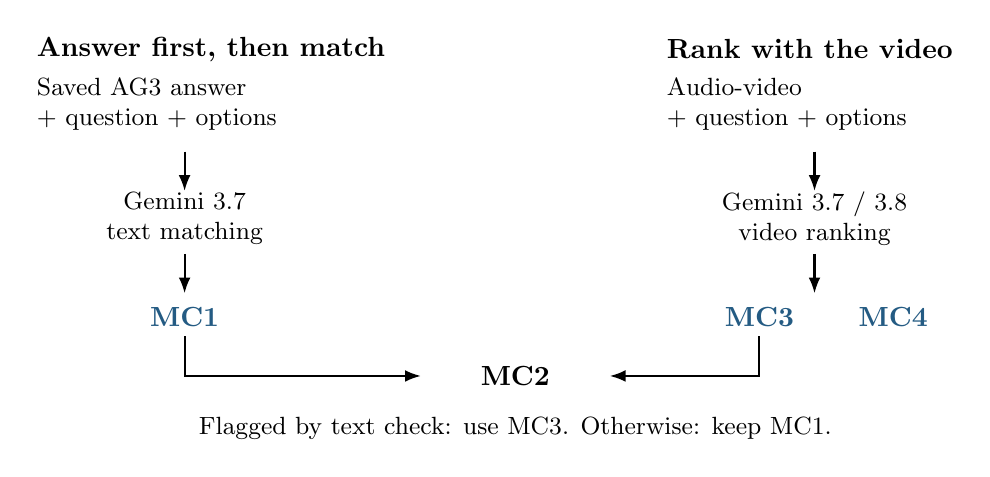
\begin{tikzpicture}[font=\small]
\node[anchor=west,font=\bfseries] at (0,.6) {Answer first, then match};
\node[anchor=west,font=\bfseries] at (8,.6) {Rank with the video};
\node[anchor=west,align=left] at (0,-.1) {Saved AG3 answer\\+ question + options};
\node[anchor=west,align=left] at (8,-.1) {Audio-video\\+ question + options};
\draw[flowarrow] (2,-.7)--(2,-1.2);
\draw[flowarrow] (10,-.7)--(10,-1.2);
\node[align=center] at (2,-1.55) {Gemini 3.7\\text matching};
\node[align=center] at (10,-1.55) {Gemini 3.7 / 3.8\\video ranking};
\draw[flowarrow] (2,-2)--(2,-2.5);
\draw[flowarrow] (10,-2)--(10,-2.5);
\node[font=\bfseries,text=evidenceblue] (m1) at (2,-2.8) {MC1};
\node[font=\bfseries,text=evidenceblue] (m3) at (9.3,-2.8) {MC3};
\node[font=\bfseries,text=evidenceblue] at (11,-2.8) {MC4};
\draw[flowarrow] (m1.south)--(2,-3.55)--(5,-3.55);
\draw[flowarrow] (m3.south)--(9.3,-3.55)--(7.4,-3.55);
\node[font=\bfseries] at (6.2,-3.55) {MC2};
\node[anchor=north,align=center] at (6.2,-3.95) {Flagged by text check: use MC3. Otherwise: keep MC1.};
\end{tikzpicture}
\caption{Video calls receive no saved AG answer. MC2 reuses MC3 predictions, not MC4's. Any invalid or unavailable video ranking falls back to MC1.}\label{fig:mc}
\end{figure}
The text check flags partial or absent matches, requests to see video, or an MC1 choice outside the checker's closest matches. It selects 798 questions; 786 receive valid MC3 rankings. This is a comparison of saved predictions, not measured computation savings. Model settings and fallbacks are in Appendix~\ref{app:settings}.

\clearpage
\section{Results: gains come with new errors}
\subsection{AG: the largest difference is in METEOR}
\begin{figure}[H]\centering
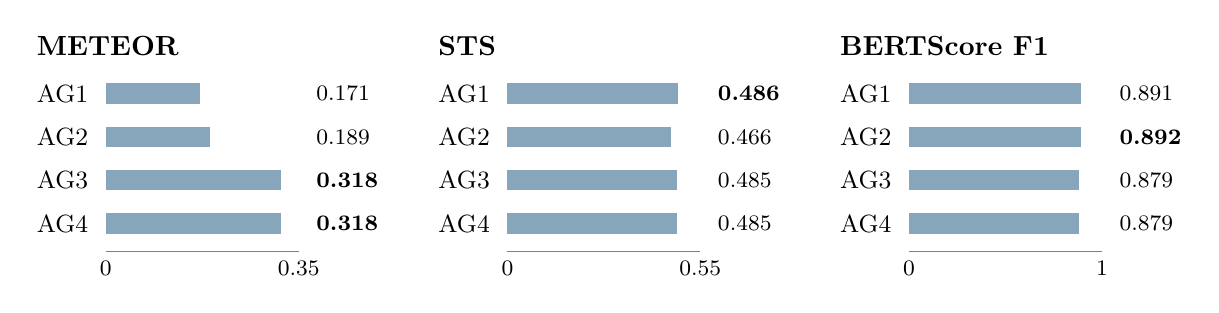
\begin{tikzpicture}[font=\small,x=1cm,y=1cm]
\node[anchor=west,font=\bfseries] at (0.0,.6) {METEOR};
\node[anchor=west] at (0.0,0.0) {AG1};\fill[evidenceblue!55] (1.0,-0.13) rectangle (2.193759,0.13);\node[anchor=west,font=\footnotesize] at (3.55,0.0) {0.171};
\node[anchor=west] at (0.0,-0.55) {AG2};\fill[evidenceblue!55] (1.0,-0.68) rectangle (2.3200460000000005,-0.42000000000000004);\node[anchor=west,font=\footnotesize] at (3.55,-0.55) {0.189};
\node[anchor=west] at (0.0,-1.1) {AG3};\fill[evidenceblue!55] (1.0,-1.23) rectangle (3.2277080000000002,-0.9700000000000001);\node[anchor=west,font=\footnotesize] at (3.55,-1.1) {\textbf{0.318}};
\node[anchor=west] at (0.0,-1.6500000000000001) {AG4};\fill[evidenceblue!55] (1.0,-1.7800000000000002) rectangle (3.2277080000000002,-1.52);\node[anchor=west,font=\footnotesize] at (3.55,-1.6500000000000001) {\textbf{0.318}};
\draw[gray] (1.0,-2)--(3.45,-2);\node[below,font=\footnotesize] at (1.0,-2) {0};\node[below,font=\footnotesize] at (3.45,-2) {0.35};
\node[anchor=west,font=\bfseries] at (5.1,.6) {STS};
\node[anchor=west] at (5.1,0.0) {AG1};\fill[evidenceblue!55] (6.1,-0.13) rectangle (8.262913454545455,0.13);\node[anchor=west,font=\footnotesize] at (8.649999999999999,0.0) {\textbf{0.486}};
\node[anchor=west] at (5.1,-0.55) {AG2};\fill[evidenceblue!55] (6.1,-0.68) rectangle (8.175051999999999,-0.42000000000000004);\node[anchor=west,font=\footnotesize] at (8.649999999999999,-0.55) {0.466};
\node[anchor=west] at (5.1,-1.1) {AG3};\fill[evidenceblue!55] (6.1,-1.23) rectangle (8.258347545454544,-0.9700000000000001);\node[anchor=west,font=\footnotesize] at (8.649999999999999,-1.1) {0.485};
\node[anchor=west] at (5.1,-1.6500000000000001) {AG4};\fill[evidenceblue!55] (6.1,-1.7800000000000002) rectangle (8.258347545454544,-1.52);\node[anchor=west,font=\footnotesize] at (8.649999999999999,-1.6500000000000001) {0.485};
\draw[gray] (6.1,-2)--(8.55,-2);\node[below,font=\footnotesize] at (6.1,-2) {0};\node[below,font=\footnotesize] at (8.55,-2) {0.55};
\node[anchor=west,font=\bfseries] at (10.2,.6) {BERTScore F1};
\node[anchor=west] at (10.2,0.0) {AG1};\fill[evidenceblue!55] (11.2,-0.13) rectangle (13.38230565,0.13);\node[anchor=west,font=\footnotesize] at (13.75,0.0) {0.891};
\node[anchor=west] at (10.2,-0.55) {AG2};\fill[evidenceblue!55] (11.2,-0.68) rectangle (13.384500849999998,-0.42000000000000004);\node[anchor=west,font=\footnotesize] at (13.75,-0.55) {\textbf{0.892}};
\node[anchor=west] at (10.2,-1.1) {AG3};\fill[evidenceblue!55] (11.2,-1.23) rectangle (13.353224149999999,-0.9700000000000001);\node[anchor=west,font=\footnotesize] at (13.75,-1.1) {0.879};
\node[anchor=west] at (10.2,-1.6500000000000001) {AG4};\fill[evidenceblue!55] (11.2,-1.7800000000000002) rectangle (13.353224149999999,-1.52);\node[anchor=west,font=\footnotesize] at (13.75,-1.6500000000000001) {0.879};
\draw[gray] (11.2,-2)--(13.649999999999999,-2);\node[below,font=\footnotesize] at (11.2,-2) {0};\node[below,font=\footnotesize] at (13.649999999999999,-2) {1};
\end{tikzpicture}
\caption{Official rank-one similarity on 2,428 questions, using human plus alternative references. Each metric has its own labeled scale. Bold values lead that metric; these are not accuracy scores. Exact values appear in Appendix~\ref{app:scores}.}\label{fig:agresults}
\end{figure}
AG3/AG4 lead METEOR; the best STS and BERTScore runs are separated from the next run by about .001. The pattern also holds with human-only references. AG4 keeps rank one unchanged but its overall ranked-list score is lower: METEOR NDCG@10 falls from .862 to .813. Both wording and order change, so this does not isolate a cause. Comparisons are descriptive, without significance testing.

\subsection{MC: more video rankings, higher accuracy}
\begin{figure}[H]\centering
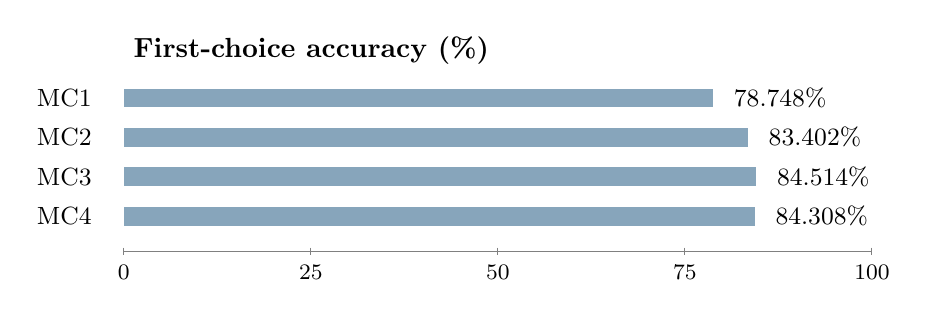
\begin{tikzpicture}[font=\small,x=.095cm,y=1cm]
\foreach \y/\id/\v in {0/MC1/78.748,-.5/MC2/83.402,-1/MC3/84.514,-1.5/MC4/84.308} {
 \node[anchor=east] at (-3,\y) {\id};
 \fill[evidenceblue!55] (0,\y-.12) rectangle (\v,\y+.12);
 \node[anchor=west] at (\v+1.5,\y) {\v\%};}
\draw[gray] (0,-1.95)--(100,-1.95);
\foreach \x in {0,25,50,75,100} {\draw[gray] (\x,-1.9)--(\x,-2);\node[below,font=\footnotesize] at (\x,-2) {\x};}
\node[anchor=west,font=\bfseries] at (0,.6) {First-choice accuracy (\%)};
\end{tikzpicture}
\caption{MC3 has 2,052 correct answers, six fewer than the leaderboard leader. Other teams' question-level results were unavailable.}\label{fig:mcresults}
\end{figure}
\begin{figure}[H]\centering
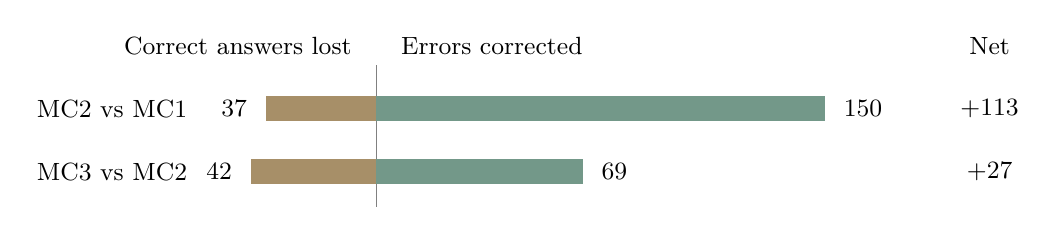
\begin{tikzpicture}[x=.038cm,y=1cm,font=\small]
\node[anchor=east] at (-5,.5) {Correct answers lost};
\node[anchor=west] at (5,.5) {Errors corrected};
\node at (205,.5) {Net};
\draw[gray] (0,.25)--(0,-1.55);
\foreach \y/\left/\right/\net/\label in {-.3/37/150/113/MC2 vs MC1,-1.1/42/69/27/MC3 vs MC2} {
 \fill[reviewamber!65] (-\left,\y-.16) rectangle (0,\y+.16);
 \fill[decisiongreen!65] (0,\y-.16) rectangle (\right,\y+.16);
 \node[anchor=east] at (-\left-3,\y) {\left};
 \node[anchor=west] at (\right+3,\y) {\right};
 \node at (205,\y) {+\net};
 \node[anchor=east] at (-60,\y) {\label};}
\end{tikzpicture}
\caption{Paired changes on the same questions. MC3 expands the use of the same video predictions used by MC2: 69 extra corrections come with 42 new errors.}\label{fig:changes}
\end{figure}
\textbf{Counting remains difficult.} On 309 ``how many'' questions, MC3 gets 200 right, versus MC2's 205 and MC4's 204. Of MC3's 109 misses, 76 choose an explicit number different from the official option. This lexical analysis identifies disagreements, not their causes.

\clearpage
\section{One question: wording, grouping, and choice}
\label{sec:worked}
\begin{minipage}{.36\linewidth}\centering
\includegraphics[width=\linewidth]{private-frames/weather-02.jpg}
\end{minipage}\hfill
\begin{minipage}{.60\linewidth}\raggedright
\textbf{``What is the weather like when someone is filming the white building?''}\\[5pt]
Q\_ID 1835; \run{8083.webm}; frame at 2 s.\\[5pt]
\textbf{Official MC answer: Sunny.}\\
{\small Frames illustrate clips, not reconstructed model inputs.}
\end{minipage}

\subsection*{A. Same meaning, different similarity score}
\begin{center}\small
\begin{tabular}{llrrr}\toprule
Run & First answer & STS & METEOR & BERTScore\\\midrule
AG1 & rainy & .552 & .000 & .999\\
AG2 & Sunny & 1.000 & .500 & 1.000\\
AG3 / AG4 & It is sunny. & 1.000 & .992 & 1.000\\\bottomrule
\end{tabular}\end{center}
``Sunny'' and ``It is sunny.'' agree but differ in METEOR. ``rainy'' conflicts with the official MC choice yet receives BERTScore .999. The AG reference texts are unavailable, so the scores do not reveal why.

\subsection*{B. Four source answers become two groups---then ten wordings}
\begin{figure}[H]\centering
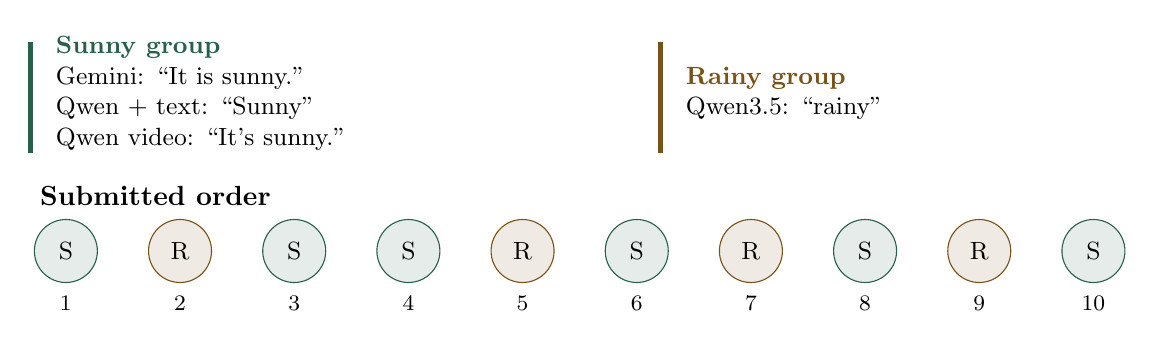
\begin{tikzpicture}[font=\small]
\draw[decisiongreen,line width=2pt] (0,0)--(0,1.4);
\node[anchor=west,align=left] at (.2,.75) {\textcolor{decisiongreen}{\textbf{Sunny group}}\\Gemini: ``It is sunny.''\\Qwen + text: ``Sunny''\\Qwen video: ``It's sunny.''};
\draw[reviewamber,line width=2pt] (8,0)--(8,1.4);
\node[anchor=west,align=left] at (8.2,.75) {\textcolor{reviewamber}{\textbf{Rainy group}}\\Qwen3.5: ``rainy''};
\node[anchor=west,font=\bfseries] at (0,-.55) {Submitted order};
\foreach \x/\r/\g/\c in {0/1/S/decisiongreen,1.45/2/R/reviewamber,2.9/3/S/decisiongreen,4.35/4/S/decisiongreen,5.8/5/R/reviewamber,7.25/6/S/decisiongreen,8.7/7/R/reviewamber,10.15/8/S/decisiongreen,11.6/9/R/reviewamber,13.05/10/S/decisiongreen} {
 \node[circle,draw=\c,fill=\c!12,minimum size=8mm] at (\x+.45,-1.25) {\g};
 \node[below,font=\footnotesize] at (\x+.45,-1.7) {\r};}
\end{tikzpicture}
\vspace{-3pt}
{\small\begin{tabularx}{\linewidth}{@{}YY@{}}
\textbf{Ranks 1--5} & \textbf{Ranks 6--10}\\[3pt]
1. \textcolor{decisiongreen}{[S]} It is sunny. \textit{(source; fixed first)} & 6. \textcolor{decisiongreen}{[S]} The weather is sunny.\\
2. \textcolor{reviewamber}{[R]} rainy \textit{(source)} & 7. \textcolor{reviewamber}{[R]} It is raining.\\
3. \textcolor{decisiongreen}{[S]} Sunny \textit{(source)} & 8. \textcolor{decisiongreen}{[S]} Bright and sunny.\\
4. \textcolor{decisiongreen}{[S]} It's sunny. \textit{(source)} & 9. \textcolor{reviewamber}{[R]} Rainy weather.\\
5. \textcolor{reviewamber}{[R]} The weather is rainy. & 10. \textcolor{decisiongreen}{[S]} Sunny weather.\\
\end{tabularx}}
\caption{Recorded AG4 groups and all ten answers. S = sunny; R = rainy. Answers without a source tag are added variants. Group sizes and interleaving are generated, not fixed quotas.}\label{fig:shared}
\end{figure}

\subsection*{C. Video ranking disagrees with the saved answer}
{\small\textbf{Choices:} Sunny; Partly cloudy; Cloudy; Windy; Foggy; Rainy; Stormy; Snowy. Display order follows MC1's ranking.}
\begin{center}\small
\textcolor{decisiongreen}{\textbf{MC1 / MC2 / MC4: Sunny}}\qquad
\textcolor{reviewamber}{\textbf{MC3: Rainy}}\\[3pt]
Sunny ranks first in MC1/MC2/MC4 and seventh in MC3.
\end{center}
MC1 matches AG3's saved ``It is sunny.''; MC3 ranks from video without that answer. MC1, MC2, and MC4 are correct while MC3 is wrong on 20 of 2,428 questions, including this one. MC3 still gains 140 correct choices over MC1 overall; this case does not explain why the predictions differ.

\clearpage
\section{When different choices mean the same answer}
All four MC runs miss the same \textbf{271 questions}. We screened their questions, options, and predictions, then inspected eight selected clips. Two cases reveal equivalent choices that receive different scores.
\label{sec:shared-errors}
\begin{figure}[H]\centering
\includegraphics[width=.65\linewidth]{private-frames/hat-50.jpg}\\[5pt]
{\small Q\_ID 2049; \run{Archipelago-42.webm}; 50 s}\par
\medskip
\textbf{``How many people in the video are wearing a hat?''}

\begin{tikzpicture}[font=\small]
\node[anchor=north,align=center,text width=6cm] at (3,0) {\textcolor{decisiongreen}{\textbf{Official choice}}\\[5pt]{\Large ``One''}\\[5pt]Scored correct};
\node[anchor=north,align=center,text width=6cm] at (10.5,0) {\textcolor{evidenceblue}{\textbf{All four runs choose}}\\[5pt]``One person is wearing a hat''\\[5pt]Scored wrong};
\draw[gray, line width=.8pt] (3,-1.8)--(3,-2.1)--(10.5,-2.1)--(10.5,-1.8);
\node[anchor=north,font=\bfseries] at (6.75,-2.25) {Same count; different option strings};
\end{tikzpicture}
\caption{Both wordings are organizer-provided choices. Every run puts the longer answer first and the designated choice second.}
\end{figure}
\medskip\hrule\medskip
\textbf{The same issue appears in the bed-count question.}\\
``How many beds are in the house?''\quad {\small Q\_ID 1369; \run{Memphis-18.webm}}
\begin{center}
\textcolor{decisiongreen}{Official: ``One''}\qquad$\equiv$\qquad
\textcolor{evidenceblue}{All four runs: ``One bed''}
\end{center}
More video evidence cannot distinguish these two answers by meaning. These cases show a mismatch with the designated option, not evidence that the underlying count is wrong. The targeted review does not estimate prevalence, and other teams' question-level errors were unavailable.

\textbf{Overall takeaway.} Broader video ranking improves MC accuracy while introducing new errors. AG scores depend on the metric, and ten distinct strings need not represent ten distinct answers.

\clearpage
\appendix
\section{Exact scores and implementation details}
\label{app:scores}
\begingroup\small
\begin{center}
\begin{tabular}{lrrr}
\toprule
Run & STS@1 & METEOR@1 & BERTScore F1@1\\
\midrule
AG1 --- \run{q35_4b_u12} & .485552 & .170537 & .890737\\
AG2 --- \run{q36_dualview} & .465828 & .188578 & .891633\\
AG3 --- \run{g37_q36_fusion} & .484527 & .318244 & .878867\\
AG4 --- \run{g37_grouped_unique} & .484527 & .318244 & .878867\\
\bottomrule
\end{tabular}
\end{center}
\begin{center}
\begin{tabular}{lrrr}
\toprule
Run & Correct / 2,428 & Accuracy & MRR\\
\midrule
MC1 --- \run{g37q36_mc_text} & 1912 & 78.748\% & .864605\\
MC2 --- \run{g37_mc_target} & 2025 & 83.402\% & .896845\\
MC3 --- \run{g37_mc_direct} & 2052 & 84.514\% & .905653\\
MC4 --- \run{g38_mc_direct} & 2047 & 84.308\% & .905368\\
\bottomrule
\end{tabular}
\end{center}
Official scores use the same 2,428 questions~\cite{official2026}. AG uses human plus alternative references; MC reports correct counts, accuracy, and mean reciprocal rank (MRR). NDCG measures discounted relevance across AG's ranked list.

\label{app:settings}
\textbf{Settings and fallbacks.} AG1 samples 12 interval midpoints, requests repairs for short lists, then uses generic fillers (650 of 24,430 positions). Ten unavailable-video rows use the question alone and are excluded from scoring. AG2 uses Qwen3.6-27B at temperature zero, thinking disabled, and 64 output tokens; its video path is not assumed to consume native audio. AG3 uses Gemini 3.7 Flash at 4 fps, low resolution, high thinking, and 2,048 output tokens. MC3 uses the same frame rate, resolution, and thinking setting. MC2 has 786 valid replacements and 12 selected fallbacks. MC3 has 2,423 valid video rankings and 20 fallbacks; MC4 has 2,428 and 15. These are submission counts before exclusions.

\textbf{A source-priority disagreement.} Q\_ID 106 (\run{8008.webm}) asks how many people are shown. A 1-fps inspection shows two, matching the official MC answer. AG3 says ``4 people (two main subjects and two partially visible in the foreground).'' We did not find those additional people in the inspected frames. AG1's ``2'' remains at rank three in AG3. MC1/2/3 choose four; MC4 chooses two. The inspection does not establish a sampling cause.

\textbf{Counting analysis.} The ``how many'' group is a lexical screen, not an organizer annotation. Numeric disagreements compare digits and number words zero--twenty, excluding vague quantities.

\textbf{Why we tried transcripts.} On 30 labeled 2025 examples, adding quality-checked Whisper large-v3 text to the same Qwen3.5-4B frames raises exact matches from 9 to 11 and mean token F1 from .431 to .507. The panel has six examples each for speech, sound/music, temporal actions, spatial/OCR/color, and visual controls. Speech token F1 rises from .431 to .700; neither condition exactly answers a sound/music question. Exact match compares normalized strings; token F1 measures token overlap. AG2 also changes the model and video input, so this development comparison does not isolate AG2's test-set differences.

\textbf{Audit boundary.} We checked the shared failures against original options and frozen rankings. Beyond the two equivalent-choice cases, inspected clips had timing ambiguity, unclear details, or potentially synonymous options. Those cases remain unresolved; selection was not random. Detailed records remain in the supporting analysis.
\endgroup

\begingroup\small\raggedright
\begin{thebibliography}{9}
\setlength{\itemsep}{0pt}
\bibitem{guidelines2026} NIST. \emph{TRECVID 2026: Video Question Answering guidelines}. \url{https://www-nlpir.nist.gov/projects/tv2026/vqa.html}.
\bibitem{smeaton2006} A. F. Smeaton, P. Over, and W. Kraaij. Evaluation campaigns and TRECVid. \emph{MIR}, 2006, pp. 321--330. \href{https://doi.org/10.1145/1178677.1178722}{doi:10.1145/1178677.1178722}.
\bibitem{official2026} NIST. \emph{TREC VQA 2026 evaluation results}. Participant release, September 2026. AG workbook and NP Labs MC scores; archived at repository revision \run{3efb5b19dbd6d8d59232986cc25ef049af24ba5e}.
\end{thebibliography}
\endgroup

{\small\textbf{Drafting assistance.} Codex assisted with writing, figures, and source checks. Author review and final model references remain to be completed.}
\end{document}
